\documentclass[12pt]{book}

\usepackage{tabularx}
\usepackage{tikz} 

\usepackage{epigraph}


\usetikzlibrary{shapes}
\usetikzlibrary{arrows}
\usetikzlibrary{positioning}
\usetikzlibrary{patterns}
\usepackage[margin=1.1in,footskip=.25in]{geometry}
\usepackage{amsmath, amssymb}
\usepackage{mathtools}
\renewcommand{\baselinestretch}{1.3} 
\usepackage[most]{tcolorbox}



\tcbset{
    frame code={}
    center title,
    left=10pt,
    right=10pt,
    top=10pt,
    bottom=10pt,
    colback=gray!5,
    colframe=gray,
    width=\dimexpr\textwidth\relax,
    enlarge left by=0mm,
    boxsep=5pt,
    arc=0pt,outer arc=0pt,
}






\renewcommand\epigraphflush{flushright}
\renewcommand\epigraphsize{\normalsize}
\setlength\epigraphwidth{0.7\textwidth}

\definecolor{titlepagecolor}{cmyk}{1,.60,0,.40}

\DeclareFixedFont{\titlefont}{T1}{ppl}{b}{it}{0.5in}


\newcommand\titlepagedecoration{%
\begin{tikzpicture}[remember picture,overlay,shorten >= -10pt]

\coordinate (aux1) at ([yshift=-15pt]current page.north east);
\coordinate (aux2) at ([yshift=-410pt]current page.north east);
\coordinate (aux3) at ([xshift=-4.5cm]current page.north east);
\coordinate (aux4) at ([yshift=-150pt]current page.north east);

\begin{scope}[titlepagecolor!40,line width=12pt,rounded corners=12pt]
\draw
  (aux1) -- coordinate (a)
  ++(225:5) --
  ++(-45:5.1) coordinate (b);
\draw[shorten <= -10pt]
  (aux3) --
  (a) --
  (aux1);
\draw[opacity=0.6,titlepagecolor,shorten <= -10pt]
  (b) --
  ++(225:2.2) --
  ++(-45:2.2);
\end{scope}
\draw[titlepagecolor,line width=8pt,rounded corners=8pt,shorten <= -10pt]
  (aux4) --
  ++(225:0.8) --
  ++(-45:0.8);
\begin{scope}[titlepagecolor!70,line width=6pt,rounded corners=8pt]
\draw[shorten <= -10pt]
  (aux2) --
  ++(225:3) coordinate[pos=0.45] (c) --
  ++(-45:3.1);
\draw
  (aux2) --
  (c) --
  ++(135:2.5) --
  ++(45:2.5) --
  ++(-45:2.5) coordinate[pos=0.3] (d);   
\draw 
  (d) -- +(45:1);
\end{scope}
\end{tikzpicture}%
}


\usepackage{xepersian}
\settextfont[Scale=1]{Vazir}



\begin{document}

%\title{معادلات دیفرانسیل}
%\maketitle

\begin{titlepage}
%\noindent
\titlefont 
\begin{tikzpicture}
\begin{scope}
\node[scale=4] (b) at (2,-2) {دیفرانسیل معادلات};
\end{scope}
\end{tikzpicture}


\null\vfill
\vspace*{1cm}
\noindent
\hfill

\titlepagedecoration
\end{titlepage}


\tableofcontents

\chapter{مفاهیم و مقدمات معادلات دیفرانسیل}

\section{تعریف معادله ی دفرانسیل}

\begin{tcolorbox}
\begin{itemize}
	\item رابطه ی بین یک تابع و مشتق های آن
	\item معادله ای که خود تابع و مشتق آن تابع در آن حضور داشته باشند
\end{itemize}
\end{tcolorbox}

\begin{tcolorbox}
\begin{itemize}
	\item $\leftarrow y = 2x $ معادله
	\item $\leftarrow y \geq 2x $ نامعادله
\end{itemize}
\end{tcolorbox}

\section{انواع معادلات دیفرانسیل}

\begin{latin}
\begin{tcolorbox}
\begin{itemize}
	\item ODE : Ordinary Differential Equations
	\item PDE : Partitionary Differential Equations
\end{itemize}
\end{tcolorbox}
\end{latin}

\begin{tcolorbox}
در معادله ی دیفرانسیل نیازی نیست که حتماً تابع باشد ، اما مشاق تابع حتماً باید باشد . مثل :
\begin{itemize}
	\item $y + y' = 5$
	\item $y'' + y' = 0$
	\item $y'y'' = 7$
\end{itemize}
\end{tcolorbox}

\section{کاربرد معادلات دیفرانسیل}

\begin{tcolorbox}
\begin{itemize}
	\item سقوط آزاد اجسام
	\item به دست آوردن دمای مرکز خورشید
\end{itemize}
\end{tcolorbox}


\subsubsection{مثال}
فاصله ی گلوله در ثانیه ی t ام از مبدا چقدر است ؟

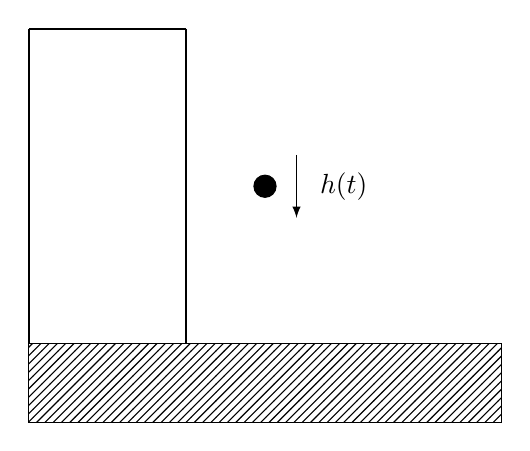
\begin{tikzpicture}[scale=2]
\draw[thick] (0,0) -- (0,2);
\draw[thick] (0,2) -- (1,2);
\draw[thick] (1,2) -- (1,0);
\draw[fill=black] (1.5,1) circle (2pt);
\draw[->,>=latex] (1.7,1.2) -- (1.7,.8) ;
\node (a) at (2,1) {$h(t)$};  
\draw[pattern=north east lines] (0,0) rectangle (3,-.5);
\end{tikzpicture}

\begin{center}
  \bgroup
  \def\arraystretch{1.5}%
  \begin{tabular}{  l  c  r }
    مکان در لحظه ی t
     & $= S =$  & $h(t)$ \\ 
    سرعت در لحظه ی t
     & $= V =$  & $h'(t) = \frac{ds}{dt}$ \\ 
    شتاب در لحظه ی t
     & $= a =$  & $h''(t) = \frac{dv}{dt} =  \frac{d^{2}s}{dt^{2}}$ \\
  \end{tabular}
  \egroup
\end{center}

\newpage

\subsubsection{مثال}
به دست آوردن شتاب گرانش ( g ) در سقوط آزاد ؟

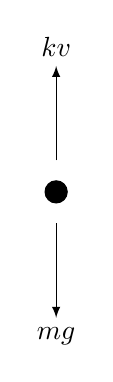
\begin{tikzpicture}[scale=2]
\draw[fill=black] (1.5,1) circle (2pt);
\draw[->,>=latex] (1.5,1.2) -- (1.5,1.8) node[above] {$kv$} ;
\draw[->,>=latex] (1.5,.8) -- (1.5,.2) node[below] {$mg$} ;
\end{tikzpicture}


\begin{align*}
\sum{F} = ma  &\to mg - kv = ma \\
 &\to mg = ma + kv \\
 &\to g = a + \frac{k}{m}v \\
 &\to g = S'_{t} + \frac{k}{m} S''_{t} \\
\end{align*}



\begin{tcolorbox}
\begin{itemize}
	\item معادلات دیفرانسیل Ordinary برای 
	توابع یک متغیره است
	\item معادلات دیفرانسیل Partitionary
	برای توابع چند متغیره است که دارای مشتق ضمنی با جزیی هستند
\end{itemize}
\end{tcolorbox}



\begin{tcolorbox}
نماد معادلات دیفرانسیل معمولی
\begin{itemize}
	\item $F ( x , y' , y'' , \dots , y^{n} ) = 0$
\end{itemize}
\end{tcolorbox}


\newpage

\section{مرتبه ی معادلات دیفرانسیل}

بالاترین مرتبه ی مشتق موجود در معادله ی دیفرانسیل را مرتبه ی معادله ی دیفرانسیل می نامیم .


\begin{center}
  \bgroup
  \def\arraystretch{1.5}%
  \begin{tabular}{  c | c | c | c }
    $y' = \cos{x}$ & خطی
     & درجه 1
      & مرتبه 1  \\ 
    $y' = \cfrac{1}{1+x^{2}}$ & خطی
     & درجه 1
      & مرتبه 1 \\ 
    $y'' + y = x$ & خطی
     & درجه 1
      & مرتبه 2 \\ 
    $y'' + (3y')^{3} + 2x = 5$ & غیر خطی
     & درجه 1
      & مرتبه 2 \\
    $(y''')^{3} + (y'')^{4} + y' = x$ & غیر خطی
     & درجه 3
      & مرتبه 3 \\
    $x^{2}y'' + \sin{y'} = x^{2} + 1$ & غیر خطی
     & درجه 1
      & مرتبه 2 \\
  \end{tabular}
  \egroup
\end{center}


\section{تعریف خطی بودن}

معادله ی دیفرانسیل به فرم :

$$
a_{n}(x) y^{n} + a_{n-1}(x) y^{n-1} + \dots + a_{1}(x) y^{1} + a_{0}(x)y = g(x)
$$

خطی نامیده می شود به شرطی که در آن ضرایب $a(x)$ فقط بر حسب x  باشند .

\subsubsection{مثال}
معادله ی دیفرانسیل زیر غیر خطی است . زیرا ضرایب فقط بر حسب x نیست .

$$
y''' + \underbrace{2y} y'' + y = 2x 
$$


\subsubsection{مثال}
معادله ی دیفرانسیل زیر غیر خطی است . زیرا مشتق توان بیشتر از 1 یا توان منفی نباید داشته باشد .

$$
\underbrace{(y''')^{2}} + 2x y'' + y = 2x 
$$

\subsubsection{مثال}
معادله ی دیفرانسیل زیر خطی است . 

$$
y'' + x y'  = 4x
$$


\section{درجه ی معادله ی دیفرانسیل}

توان بالاترین مشتق ( توان مرتبه ) ، درجه ی معادله ی دیفرانسیل نامیده می شود .


\begin{tcolorbox}
فرق چند جمله ای و چند ضابطه ای
\begin{itemize}
	\item معادله ی زیر یک چند جمله ای است
	$$
	f(x) = 3x^{5} + 4x^{2} + 5
	$$
	\item معادله ی زیر یک چند ضابطه ای است 
	اما چند جمله ای نیست ، چون در چند جمله ای x باید آزاد باشد
	$$
	f(x) = \sin{x} + \sqrt{x} + \frac{1}{x} - 2
	$$
\end{itemize}
\end{tcolorbox}


\section{مفهوم دسته منحنی}

در معادله ی 
$$
y = F(x,c)
$$

به ازای مقادیر مختلفی که c اختیار می کند ، منحنی های بی شماری رسم می شوند ، به این دلیل به آن دسته منحنی می گوییم .

\newpage
\section{جواب معادله دیفرانسیل}

هر تابعی که در معادله ی دیفرانسیل صدق کند جواب آن نامیده می شود .

\begin{align*}
y' = \cos{x} &\to  y = \sin{x} \\
y'' + y = x &\to y = x \\
\end{align*}


\section{انواع جواب معادله ی دیفرانسیل}


\begin{tcolorbox}
\begin{itemize}
	\item جواب عمومی :
	یک خانواده ی n پارامتری از جوابهای یک معادله ی دیفرانسیل مرتبه ی n ام .
	
	\item جواب خصوصی : 
	با مقدار دهی به پارامتر ها می توان جواب خصوصی معادله ی دیفرانسیل را به دست آورد .
	
	\item جواب غیر عادی :
	منحنی نمایش آن بر تمام منحنی های جواب عمومی مماس باشد .
\end{itemize}
\end{tcolorbox}


\section{متغیر مستقل و متغیر وابسته}

در تابع 
$$
y = f(x)
$$

به x  متغیر مستقل و به y متغیر وابسته می گوییم .

\chapter{معادلات دیفرانسیل مرتبه ی اول}

به معادلات دیفرانسیل به فرم کلی
$$
F(x,y,y') = 0
$$

معادلات دیفرانسیل مرتبه ی اول می گوییم .

\begin{center}
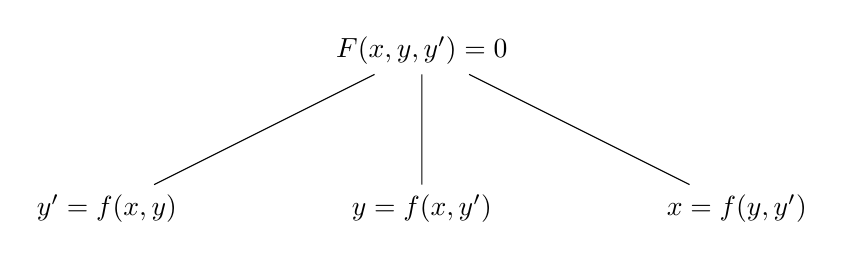
\begin{tikzpicture}[node distance = 1cm,level distance = 2cm,sibling distance = 4cm]
\node {$F(x,y,y') = 0$}
child {node {$y' = f(x,y)$}}
child {node {$y = f(x,y')$}}
child {node {$x = f(y,y')$}
};
\end{tikzpicture}
\end{center}


\section{انواع معادلات دیفرانسیل مرتبه ی اول}

\begin{tcolorbox}
\begin{itemize}
	\item مجزا ( جدا شدنی )
	\item همگن
	\item کامل
	\item خطی مرتبه ی اول
	\item خطی مرتبه ی دوم
\end{itemize}
\end{tcolorbox}


\section{روال حل معادلات دیفرانسیل}

\begin{tcolorbox}
\begin{itemize}
	\item تشخیص 
	\item حل
\end{itemize}
\end{tcolorbox}


\section{معادلات دیفرانسیل جدا شدنی}

اگر
$y' = f(x,y)$
را بتوان به صورت 
$$
f(x)dx + g(y)dy = 0
$$
نوشت ، در این صورت به آن معادله ی جداشدنی می گویند .
برای به دست آوردن جواب عمومی این معادله ی دیفرانسیل کافی است از طرفین معادله انتگرال بگیریم .
$$
\int{f(x)dx} + \int{g(y)dy} = \int{0}
$$


\section{روش های حل انتگرال}

\begin{tcolorbox}
\begin{itemize}
	\item از طریق مشتق
	\item جز به جز
	$$
	\int{fg'} = fg - \int{f'g}
	$$
	\item تجزیه ی کسر ها
	\item تغییر متغیر
	\begin{align*}
	y^{2} &= u \\
	2ydy &= du \\
	\end{align*}
\end{itemize}
\end{tcolorbox}

\subsubsection{مثال}

$$
y' = \frac{x}{y}
$$

\begin{align*}
y' = \frac{x}{y} &\to \frac{dy}{dx} = \frac{x}{y} \\
&\to ydy = xdx \\
&\to  \int{ydy} = \int{xdx} \\
&\to \frac{y^{2}}{2} = \frac{x^{2}}{2} + C \\
&\to y^{2} = 2 \left( \frac{x^{2}}{2} + C \right) = x^{2} + 2C \\
&\to y^{2} = x^{2} + 2C 
\end{align*}


\begin{tcolorbox}
نکته :
\begin{itemize}
	\item 
	$$
	\int {x^{n} dx} = \frac{x^{n+1}}{n+1} + C
	$$
\end{itemize}
\end{tcolorbox}


\subsubsection{مثال}

$$
y' = \frac{2x+xy}{x^{2}+4}
$$

\begin{align*}
y' = \frac{2x + xy}{x^{2}+4} &\to \frac{dy}{dx} = \frac{x(y+2)}{x^{2}+4} \\
&\to \frac{dy}{y+2} = \frac{xdx}{x^{2}+4} \\
&\to \int{\frac{dy}{y+2}} = \int{\frac{xdx}{x^{2}+4}} \\
&\to x^{2} + 4 = u \\
&\to 2xdx = du \\
&\to xdx = \frac{1}{2} du \\
&\to \int{\frac{dy}{y+2}} = \int{\frac{1}{2} \frac{du}{u} } \\
&\to \ln{(y+2)} = \frac{1}{2} \left( \ln{u} + \ln{c} \right) \\
&\to \ln{(y+2)} = \frac{1}{2} \left( \ln{cu} \right) \\
&\to \ln{(y+2)} = \ln{(cu)^{\frac{1}{2}}} \\
&\to y+2 = \sqrt{cu} \\
&\to y + 2 = \sqrt{c(x^{2}+4)}
\end{align*}



\subsubsection{مثال}

$$
e^{y^{2}} ( x^{2} + 2x + 1 ) = - ( xy + y ) y' 
$$


\begin{align*}
&\to e^{y^{2}} ( x + 1 )^{2} = - (x+1) yy' \\
&\to e^{y^{2}} (x + 1) = - y \frac{dy}{dx} \\
&\to (x+1)dx = \frac{-ydy}{e^{y^{2}}} \\
&\to y^{2} = u \\
&\to 2ydy = du \\
&\to ydy = \frac{1}{2} du \\
&\to - ydy = - \frac{1}{2} du \\
&\to (x+1)dx = - \frac{1}{2} \frac{du}{e^{u} } \\
&\to (x+1)dx = - \frac{1}{2} e^{-u} du \\
&\to xdx + dx = - \frac{1}{2} e^{-u} du \\
&\to \int{xdx} + \int{dx} = \int{- \frac{1}{2} e^{-u} du} \\
&\to \frac{x^{2}}{2} + x = - \frac{1}{2} - e^{-u} + C \\
&\to \frac{x^{2}}{2} + x =  \frac{1}{2}  e^{-u} + C \\
&\to u = y^{2} \\
&\to \frac{x^{2}}{2} + x =  \frac{1}{2}  e^{- y^{2}} + C \\
&\to 2 \left( \frac{x^{2}}{2} + x - C \right) =  e^{- y^{2}} \\
&\to \ln{(x^{2} + 2x - 2C)} = \ln{e^{- y^{2}}} \\
&\to - y^{2} = \ln{(x^{2} + 2x - 2C)} \\
&\to y^{2} = - \ln{(x^{2} + 2x - 2C)}
\end{align*}


\subsubsection{مثال}

$$
y' \cot{x} = 2 + y
$$

\begin{align*}
y' \cot{x} = 2 + y &\to \frac{dy}{dx} \times \frac{\cos{x}}{\sin{x}} = 2 + y \\
&\to \frac{dy}{2+y} = \frac{\sin{x}}{\cos{x}} dx \\
&\to \cos{x} = u \\
&\to - \sin{x} dx = du \\
&\to \ln{(y+2)} = - \ln{\cos{x}} + \ln{c} \\
&\to \ln{(y+2)} = \ln{\frac{c}{\cos{x}}} \\
&\to y + 2 = \frac{c}{\cos{x}}
\end{align*}


\subsubsection{مثال}

$$
y' = \frac{(1+y^{2})}{xy(1+x^{2})}
$$


\begin{align*}
y' = \frac{(1+y^{2})}{xy(1+x^{2})} &\to \frac{dy}{dx} = \frac{(1+y^{2})}{xy(1+x^{2})} \\
&\to \frac{ydy}{1+y^{2}} = \frac{dx}{x(1+x^{2})} \\
\end{align*}

\begin{align*}
1 + y^{2} &= u & 1 + x^{2} &= w \\
2ydy &= du & 2xdx &= dw \\
ydy &= \frac{1}{2} du & -xdx &= - \frac{1}{2} dw
\end{align*}



\begin{align*}
\frac{1}{x(1+x^{2})} &= \frac{A}{x} + \frac{Bx+C}{1+x^{2}} = \frac{A + Ax^{2} + Bx^{2} + Cx}{x(1+x^{2})} = \frac{(A+B)x^{2} + Cx + A}{x(1+x^{2})} \\
&\to A = 1 \\
&\to A + B = 0 \to B = -1 \\ 
&\to C = 0 \\
&\to \frac{1}{x(1+x^{2})} = \frac{1}{x} + \frac{-x}{1+x^{2}} \\
\end{align*}

\begin{align*}
\frac{ydy}{1+y^{2}} &= \frac{dx}{x} - \frac{xdx}{1+x^{2}} = \frac{1}{2} \frac{du}{u} = \frac{dx}{x} - \frac{1}{2} \frac{dw}{w} \\
&\to \frac{1}{2} \ln{u} = \ln{x} - \frac{1}{2} \ln{w} \\
&\to \frac{1}{2} \ln{(1+y^{2})} = \ln{x} - \frac{1}{2} \ln{1+x^{2}} \\
&\to \ln{\sqrt{1+y^{2}}} + \ln{\sqrt{1+x^{2}}} = \ln{x} \\
&\to  \ln{\sqrt{1+y^{2}} \sqrt{1+x^{2}}} = \ln{x} \\
&\to \sqrt{1+y^{2}} \sqrt{1+x^{2}} = x \\
&\to (1+y^{2}) \times (1+x^{2}) = x^{2}
\end{align*}


\section{معادله ی دیفرانسیل مرتبه ی اول همگن}

\begin{tcolorbox}
\begin{itemize}
	\item تعریف تابع همگن :
	تابع $f(x,y)$
	یک تابع همگن از درجه ی n نامیده می شود اگر به ازای هر t مثبت در این رابطه صدق کند .
	$$
	t > 0 \to f(tx,ty) = t^{n} f(x,y)
	$$
\end{itemize}
\end{tcolorbox}


\subsubsection{مثال}

تابع زیر همگن از درجه ی 2 می باشد .


\begin{align*}
f(x,y) &= x^{2} + xy + y^{2} \\
\to f(tx,ty) &= (tx)^{2} + (tx)(ty) + (ty)^{2} \\
&= t^{2}x^{2} + t^{2}xy + t^{2}y^{2} \\
&= t^{2} \left( x^{2} + xy + y^{2} \right)  \\
&= t^{2} f(x,y)
\end{align*}


\subsubsection{نکته}

\begin{tcolorbox}
\begin{itemize}
	\item درجه ی n می تواند
	کسری یا صفر نیز باشد .
\end{itemize}
\end{tcolorbox}


\subsubsection{مثال}

همگن از درجه ی $\cfrac{1}{2}$

\begin{align*}
f(x,y) &= \sqrt{x} \sin{\frac{x}{y}} \\
f(tx,ty) &= \sqrt{tx} \sin{\frac{tx}{ty}} \\
&= \sqrt{t} \sqrt{x} \sin{\frac{x}{y}} \\
&= \sqrt{t} f(x,y) \\
&= t^{\frac{1}{2}} f(x,y) 
\end{align*}


\subsubsection{مثال}

همگن از درجه ی صفر

\begin{align*}
f(x,y) &= \frac{x}{x+y} \\
f(tx,ty) &= \frac{tx}{tx+ty} \\
&= \frac{tx}{t(x+y)} \\
&= \frac{x}{x+y} \\
&= t^{0} \frac{x}{x+y} \\
\end{align*}



\section{معادله ی دیفرانسیل همگن}

$y' = f(x,y)$ 
را همگن می نامیم هرگاه درجه ی همگنی آن صفر باشد ،
برای حل معادله ی دیفرانسیل همگن از تغییر متغیر 
$y = vx$
استفاده می کنیم ، با این تغییر متغیر ، معادله ی دیفرانسیل همگن به یک معادله دیفرانسیل مجزا تبدیل می شود .

\begin{align*}
y &= vx \\
dy &= vdx + xdv \\
\end{align*}

\subsubsection{مثال}

همگن بودن معادله ی دیفرانسیل زیر را بررسی می کنیم .

$$
2xydy + (x^{2} - y^{2})dx = 0
$$

روش اول :

\begin{align*}
2xydy + ( x^{2} - y^{2} ) dx = 0 \to 2xydy &= ( x^{2} - y^{2} ) dx  \\
\to \frac{dy}{dx} &= \frac{y^{2} - x^{2}}{2xy} \\
f(tx,ty) &= \frac{t^{2}y^{2} - t^{2}x^{2}}{2 \times tx \times ty} = \frac{t^{2} ( y^{2} - x^{2} )}{ t^{2} 2xy} \\
&=  \frac{( y^{2} - x^{2} )}{2xy} \\ 
&= t^{0}  \frac{( y^{2} - x^{2} )}{2xy} \\
&\to n = 0
\end{align*}


روش دوم :

\begin{align*}
f_{1}(x,y) = 2xy &\to f_{1}(tx,ty) = 2 tx ty \\
&= t^{2} \times 2xy \\
&=  t^{2} f_{1}(x,y) \\
&\to n = 2
\end{align*}

\begin{align*}
f_{2}(x,y) = x^{2} - y^{2} &\to f_{2}(tx,ty) = t^{2}x^{2} - t^{2}y^{2} \\
&= t^{2} ( x^{2} - y^{2} ) \\
&= t^{2} f_{2}(x,y) \\
&\to n = 2
\end{align*}




\subsubsection{مثال}


$$
2xydy + (x^{2} - y^{2})dx = 0
$$

\begin{align*}
y &= vx \\
dy &= vdx + xdv \\
\end{align*}


\begin{align*}
&2x.vx.(vsx + xdv) + (x^{2} - v^{2}x^{2})dx = 0 \\
&\to 2vx^{2} (vsx + xdv) + x^{2}dx - v^{2}x^{2}dx = 0 \\
&\to 2v^{2}x^{2}dx + 2vx^{3}dv + x^{2}dx - v^{2}x^{2}dx = 0 \\
&\to x^{2}v^{2}dx + x^{2}dx + 2vx^{3}dv = 0 \\
&\to x^{2}(1 + v^{2})dx + 2vx^{3}dv = 0 \\
&\to \frac{x^{2}}{x^{3}} dx + \frac{2v}{1+v^{2}} = 0 \\
&\to \frac{dx}{x} + \frac{2v}{1+v^{2}}dv = 0 \\
&\to \ln{x} + \ln{1+v^{2}} = \ln{c} \\
&\to \ln{x(1 + v^{2})} = \ln{c} \\
&\to x(1 + v^{2}) = c \\ 
&\to y = vx \to v = \frac{y}{x} \\
&\to x\left( 1 + (\frac{y}{x})^{2} \right) = c \\
\end{align*}


\subsubsection{مثال}


$$
(y^{2} + 2xy)dx - x^{2}dy = 0
$$

\begin{align*}
f_{1}(x,y) = y^{2} + 2xy \to f_{1}(tx,ty) &= t^{2}y^{2} + 2.tx.ty \\
&= t^{2}y^{2} + t^{2}.2xy \\
&= t^{2}( y^{2} + 2xy ) \\
&= t^{2} f_{1}(x,y)
\end{align*}

\begin{align*}
f_{2}(x,y) = - x^{2} \to f_{2}(tx,ty) &= - t^{2} x^{2} \\
&= t^{2} ( - x^{2} ) \\
&= t^{2} f_{2}(x,y)
\end{align*}

پس معادله ی دیفرانسیل همگن می باشد .

\begin{align*}
y &= vx \\
dy &= vdx + xdv \\
\end{align*}

\begin{align*}
&( (vx)^{2} + 2x.vx ) dx - x^{2} ( vdx + xdv ) = 0 \\
&\to (v^{2}x^{2} + 2vx{2})dx - vx^{2}dx - x^{3}dv = 0 \\
&\to v^{2}x^{2} dx + 2vx^{2}dx - vx^{2}dx - x^{3}dv = 0 \\
&\to v^{2}x^{2}dx + vx^{2}dx - x^{3}dv = 0 \\
&\to x^{2} ( v + v^{2} ) dx - x^{3} dv = 0 \\
&\to \div (v + v^{2}) \quad \div x^{3} \\
&\to \frac{x^{2}}{x^{3}}dx - \frac{1}{v + v^{2}}dv = 0 \\
&\to \frac{dx}{x} - \frac{dv}{v + v^{2}} \\
&\to \frac{dx}{x} - \frac{dv}{v(1+v)} = 0 \\
\end{align*}

\begin{align*}
& \frac{1}{v(1+v)} = \frac{A}{v} + \frac{B}{1+v} \\
&= \frac{A + A.v + B.v}{v(1+v)} \\
&= \frac{(A+B)v + A}{v(1+v)} \\
&\to A = 1 \\
&\to A + B = 0 \to B = -1 \\
&\to \frac{1}{v(1+v)} = \frac{1}{v} - \frac{1}{1+v}
\end{align*}


\begin{align*}
&\to \frac{dx}{x} - \left( \frac{dv}{v} - \frac{dv}{1+v} \right) = 0  \\
&\to \frac{dx}{x} -  \frac{dv}{v} + \frac{dv}{1+v} = 0  \\
&\to \ln{x} - \ln{v} + \ln{1+v} = \ln{c} \\
&\to \ln{x} + \ln{\frac{1+v}{v}} = \ln{c} \\
&\to y = v.x \to v = \frac{y}{x} \\
&\to x . \frac{1+v}{v} = c \\
&\to x + \frac{1 + \frac{y}{x}}{\frac{y}{x}} = c \\
\end{align*}


\section{معادله ی دیفرانسیل کامل}

معادله ی 
$y' = f(x,y)$
می تواند به فرم خطی 
$$
M(x,y)dx + N(x,y)dy = 0 
$$
تبدیل شود و این معادله کامل نامیده می شود اگر
$F(x,y)$
وجود داشته باشد که :
$$
\frac{\partial{F(x,y)}}{\partial{x}} = M(x,y)
$$ 

یعنی از F مشتق گرفته شده نسبت به x و شده M(x,y)

و

$$
\frac{\partial{F(x,y)}}{\partial{y}} = N(x,y)
$$

یعنی از F مشتق گرفته شده نسبت به y و شده N(x,y)


\section{جواب معادله ی دیفرانسیل کامل}

\begin{tcolorbox}
$$
F(x,y) = \int{M(x,y)dx} + \int{(N - scentences \:\: without \:\: x) dy}
$$
\end{tcolorbox}

\subsubsection{مثال}

چگونگی ساختن یک معادله ی دیفرانسیل کامل 

\begin{align*}
F(x,y) = x^{2} + xy + y^{2} \\
\frac{\partial{F}}{\partial{x}} = 2x + y \\
\frac{\partial{F}}{\partial{y}} = x + 2y \\
\end{align*}

در نتیجه معادله ی دیفرانسیل زیر یک معادله ی دیفرانسیل کامل است .

$$
(2x + y)dx + (x + 2y)dy = 0
$$


\subsubsection{نکته}

برای اینکه متوجه شویم معادله ی دیفرانسیل
$$
M(x,y)dx + N(x,y)dy = 0
$$
معادله ی دیفرانسیل کامل است ، باید تساوی زیر برقرار باشد .

$$
( M(x,y)dx ) dy = ( N(x,y)dy ) dx
$$

یعنی از M(x,y) که مشتق F نسبت به x است ، بار دیگر نسبت به y مشتق می گیریم .

و از N(x,y) که مشتق F نسبت به y است ، بار دیگر نسبت به x مشتق میگیریم .

و این دو باید با هم برابر باشند .

\subsubsection{مثال}

$$
( -3x^{2}y + \sin{x} )dx - ( x^{3} y )dy = 0
$$

\begin{align*}
& M(x,y) = - 3x^{2}y + \sin{x} \to \frac{\partial{M}}{\partial{y}} = -3x^{2} \\
& N(x,y) = - x^{3} - y \to \frac{\partial{N}}{\partial{x}} = - 3x^{2} 
\end{align*}

$$
F(x,y) = \int{M(x,y)dx} + \int{(N - scentences \:\: without \:\: x) dy}
$$

\begin{align*}
& \int{e^{x} \sin{y} dx} - \int{3x^{2} dx} + \int{\frac{1}{3} y^{\frac{-1}{3}} dy } \\
&= \sin{y} e^{x} - 3 \times  \frac{x^{3}}{3} + \frac{1}{3} \times \frac{y^{\frac{-2}{3} + 1}}{\frac{-2}{3} + 1} + C \\
&= e^{x} . \sin{y} - x^{3} + \frac{1}{3} \times \frac{y^{\frac{1}{3}}}{\frac{1}{3}} + C = F(x,y) 
\end{align*}


\section{معادله ی دیفرانسیل خطی مرتبه ی اول}

$$
a_{1}(x)y' + a_{2}(x)y = r(x)
$$

\begin{tcolorbox}
2 شرط برای خطی بودن :
\begin{itemize}
	\item مشتق ها توانشان 1 باشد .
	\item تمام ضرایب مشتق بر حسب x باشد .
\end{itemize}
\end{tcolorbox}

برای به دست آوردن جواب عمومی باید فرم معادله را به فرم استاندارد تبدیل کنیم .

فرم معادله استاندارد به صورت زیر می باشد .

$$
y' + p(x) y = q(x)
$$

جواب معادله دیفرانسیل خطی مرتبه ی اول در صورتی که معادله را به صورت استاندارد در بیاوریم به صورت زیر می باشد .

\begin{tcolorbox}
$$
y(x) = e^{- \displaystyle\int{p(x)dx}} \left[ \int{q(x) e ^{ {\displaystyle\int{p(x)dx}}}dx } + C \right]
$$
\end{tcolorbox}


\subsubsection{مثال}

$$
y' - xy = x
$$

این معادله استاندارد است و داریم :

$$
p(x) = -x \quad q(x) = x
$$

\begin{align*}
y(x) &= e^{- \displaystyle\int{p(x)dx}} \left[ \int{q(x) e ^{ {\displaystyle\int{p(x)dx}}}dx } + C \right] \\
&= e^{- \displaystyle\int{ - x dx}} \left[ \int{ x  e ^{ {\displaystyle\int{ - x dx}}}dx } + C \right] \\
&= e^{\frac{x^{2}}{2}} \left[ \int{ x  e ^{- \frac{x^{2}}{2}} dx } + C \right] \\
\end{align*}


\begin{align*}
- \frac{x^{2}}{2} & = u \\
- \frac{1}{2} \times 2xdx &= du \\
- x dx &= du \\
xdx &= - du \\
\end{align*}


\begin{align*}
&= e^{- u} \left[ \int{e^{u}du} + C \right] \\
&= e^{-u} \left[ e^{u} + C \right] \\
&= e^{-u} . e^{u} + c . e^{-u} \\
&= e^{0} +  c . e^{-u} \\
&= 1 +  c . e^{-u} \\
&= 1 +  c . e^{\frac{x^{2}}{2}}
\end{align*}

\chapter{معادلات دیفرانسیل مرتبه ی دوم}


\section{معادلات دیفرانسیل خطی مرتبه ی دوم}

\begin{tcolorbox}
خطی یعنی :
\begin{itemize}
	\item توان 1
	\item ضریب بر حسب x
\end{itemize}
\end{tcolorbox}

فرم کلی معادلات دیفرانسیل خطی مرتبه ی دوم به صورت زیر می باشد .

$$
a_{2}(x)y'' + a_{1}(x)y' + a_{0}(x)y = f(x) \qquad a_{2}(x) \neq 0
$$

و فرم استاندارد آن به صورت زیر است :


$$
\frac{a_{2}(x)}{a_{2}(x)}y'' + \frac{a_{1}(x)}{a_{2}(x)}y' + \frac{a_{0}(x)}{a_{2}(x)}y = \frac{f(x)}{a_{2}(x)}
$$

\begin{tcolorbox}
$$
y'' + p(x)y' + q(x)y = r(x)
$$
\end{tcolorbox}

\begin{tcolorbox}
اگر 
$r(x) \neq 0$
می شود معادله ی دیفرانسیل مرتبه ی دوم خطی غیر همگن

اگر 
$r(x) = 0$
می شود معادله ی دیفرانسیل مرتبه ی دوم خطی همگن

\end{tcolorbox}


\subsubsection{نکته}

تابع
$y(x) = 0$
به ازای هر x ای همواره جواب معادله دیفرانسیل همگن می باشد .

\subsubsection{سوال}

آیا این معادله جواب غیرصفر دیگری هم دارد ؟

بله ، اصطلاحاً به آن ترکیب جوابها می گوییم :

\begin{tcolorbox}
$$
c_{1}y_{1}(x) + c_{2}y_{2}(x) 
$$
\end{tcolorbox}


\section{جواب معادله ی دیفرانسیل خطی مرتبه ی دوم غیر همگن}

در صورتی که
$y_{1}(x)$
جواب معادله ی دیفرانسیل
$$
y'' + p(x)y' + q(x)y = r(x)
$$

و 
$y_{2}(x)$
جواب معادله ی دیفرانسیل
$$
y'' + p(x)y' + q(x)y = 0
$$
باشد .

آنگاه جواب معادله ی دیفرانسیل مرتبه ی دوم خطی غیر همگن برابر است با 
$$
y_{1}(x) + y_{2}(x)
$$


\subsubsection{نکته}

برای به دست آوردن جواب عمومی معادله ی دیفرانسیل خطی مرتبه ی دوم باید پیش نیاز های زیر را بدانیم :

\begin{itemize}
	\item وابستگی خطی
	\item استقلال خطی
\end{itemize}


\section{تعریف وابسته خطی}

اگر دو تابع 
$f(x)$
و
$g(x)$
مضرب ثابتی از هم باشند ، در این صورت وابسته خطی نامیده می شوند .

\begin{tcolorbox}
$$
f(x) = k . g(x)
$$
\end{tcolorbox}

\subsubsection{مثال}

تابع 
$f(x) = 2x^{2}$
و
$g(x)=x^{2}$
وابسته خطی هستند زیرا
$$
2x^{2} = 2 \times x^{2}
$$


تابع 
$f(x) = e^{2x}$
و
$g(x)=e^{3x}$
مستقل خطی هستند زیرا با هیچ ضریب ثابتی با هم مساوی در نمی آیند .

\begin{tcolorbox}
\begin{itemize}
	\item می توان برای تشخیص وابستگی خطی یا استقلال خطی از دترمینان رونسکین استفاده کرد
	\item در صورتی که دترمینان رونسکین برابر با صفر نبود دو تابع مستقل خطی اند
	\item در صورتی که دترمینان رونسکین برابر با صفر بود دو تابع وابسته خطی هستند 
\end{itemize}
\end{tcolorbox}


\section{تعریف دترمینان رونسکین دو تابع}


\begin{tcolorbox}
$$
w( f \circ g ) = \begin{vmatrix}
f(x) & g(x) \\
f'(x) & g'(x)
\end{vmatrix} = f(x)g'(x) - g(x)f'(x)
$$
\end{tcolorbox}

\subsubsection{مثال}

دو تابع 
$f(x)= e^{2x}$
و
$g(x) = e^{3x}$
مستقل خطی اند زیرا :

$$
\begin{vmatrix}
e^{2x} & e^{3x} \\
2e^{2x} & 3e^{3x}
\end{vmatrix} = 3e^{5x} - 2e^{5x} = e^{5x} \neq 0
$$


دو تابع 
$f(x) = 2x^{2}$
و
$g(x) = x^{2}$
وابسته خطی اند زیرا :
$$
\begin{vmatrix}
2x^{2} & x^{2} \\
4x & 2x
\end{vmatrix} = 4x^{3} - 4x^{3} =  0
$$



\begin{tcolorbox}
دو تابع وابسته خطی هستند اگر و تنها اگر
$$
w( y_{1}(x) , y_{2}(x) ) = 0
$$
\end{tcolorbox}

\begin{tcolorbox}
دو تابع مستقل خطی هستند اگر و تنها اگر
$$
w( y_{1}(x) , y_{2}(x) ) \neq 0
$$
\end{tcolorbox}


\subsubsection{سوال}

وابستگی خطی و استقلال خطی چه کمکی برای تعیین جواب عمومی معادله دیفرانسیل مرتبه ی دوم خطی همگن یا غیر همگن می کند ؟

اگر
$y_{1}(x)$
و
$y_{2}(x)$
دو جواب مستقل خطی باشند ، جواب عمومی معادله دیفرانسیل مرتبه ی دوم خطی برابر است با :
$$
y(x) = c_{1}y_{1}(x) + c_{2}y_{2}(x)
$$



\section{معادله دیفرانسیل خطی مرتبه ی دوم با ضرایب ثابت و همگن}

$$
y'' + py' + qy = 0
$$

مثل : 
$y'' + 3y' + 5y = 0$

برای حل ابتدا معادله مشخصه ی آن را تشکیل می دهیم ( از مشتق خلاص می شویم )

\begin{align*}
&y'' + py' + qy = 0  & &y'' \to r^{2} \\
& & &y' \to r \\
&\to r^{2} + pr + q = 0 & &y \to 1\\
\end{align*}


\begin{tcolorbox}
\begin{itemize}
	\item اگر 
	$\Delta > 0$
	معادله 2 ریشه ی غیر برابر دارد
	\item اگر 
	$\Delta = 0$
	معادله 2 ریشه ی برابر دارد
	\item اگر 
	$\Delta < 0$
	معادله 2 ریشه ی مختلط دارد
\end{itemize}
\end{tcolorbox}


\begin{tcolorbox}
اگر 
	$\Delta > 0$
	باشد ، معادله مشخصه 2 ریشه ی حقیقی متمایز 
	$(r_{1} , r_{2})$
	دارد و جواب عمومی معادله دیفرانسیل مرتبه ی دوم خطی برابر است با :
\begin{align*}
\begin{rcases*}
y_{1} = e^{r_{1}x} \\
y_{2} = e^{r_{2}x}
\end{rcases*}
\Rightarrow y(x) = c_{1}e^{r_{1}x} + c_{2}e^{r_{2}x}
\end{align*}
\end{tcolorbox}


\subsubsection{مثال}

$$
y'' - y' - 6y = 0 \qquad \begin{cases} y(0) = 2 \\ y'(0) = -4 \end{cases}
$$

\begin{align*}
y'' - y' - 6y = 0 \Rightarrow r^{2} - r - 6 = 0
\end{align*}

\begin{align*}
\Delta = b^{2} - 4ac = (-1)^{2} - 4 (1)(-6) = 25
\end{align*}

\begin{align*}
r = \frac{-b \pm \sqrt{\Delta}}{2a} = \frac{-(-1) \pm \sqrt{25}}{2(1)} = \frac{1 \pm 5}{2} = \begin{cases} \cfrac{6}{2} = 3 \\ -\cfrac{4}{2} = -2 \end{cases}
\end{align*}

جواب عمومی :

\begin{align*}
\begin{rcases}
y_{1}(x) = e^{3x} \\
y_{2}(x) = e^{-2x}
\end{rcases}
\Rightarrow y(x) = c_{1}e^{3x} + c_{2}e^{-2x} 
\end{align*}

\begin{align*}
\Rightarrow y'(x) = 3c_{1}e^{3x} - 2 c_{2}e^{-2x}
\end{align*}

\begin{align*}
\begin{rcases}
y(0) = 3 \\
y'(0) = -4 
\end{rcases}
\Rightarrow 
\begin{rcases}
c_{1} + c_{2} = 3 \\
3c_{1} - 2c_{2} = -4 
\end{rcases}
\Rightarrow
\begin{rcases}
2c_{1} + 2c_{2} = 6 \\
3c_{1} - 2c_{2} = -4 
\end{rcases}
\end{align*}

\begin{align*}
5c_{1} = 2 \to c_{1} = \frac{2}{5}
\end{align*}

\begin{align*}
c_{1} + c_{2} = 3 \to \frac{2}{5} + c_{2} = 3 \to c_{2} = 3 - \frac{2}{5} = \frac{15}{5} - \frac{2}{5} \to c_{2} = \frac{13}{5}
\end{align*}


جواب خصوصی : 
\begin{align*}
y(x) = \frac{2}{5} e^{3x} + \frac{13}{5} e^{-2x}
\end{align*}


\subsubsection{مثال}

$$
y'' - 4y = 0 \begin{cases} y(0) = 0 \\ y'(0) = 3 \end{cases}
$$

\begin{align*}
r^{2} - 4 = 0 \Rightarrow r^{2} = 4 \Rightarrow r = \pm 2
\end{align*}

جواب عمومی :

\begin{align*}
\begin{rcases}
y_{1}(x) = e^{2x} \\
y_{2}(x) = e^{-2x}
\end{rcases}
\Rightarrow 
y(x) = c_{1}e^{2x} + c_{2}e^{-2x}
\end{align*}

\begin{align*}
\Rightarrow y'(x) = 2c_{1}e^{2x} - 2c_{2}e^{-2x}
\end{align*}


\begin{align*}
\begin{rcases}
y(0) = 0 \\
y'(0) = 3
\end{rcases}
\Rightarrow
\begin{rcases}
c_{1} + c_{2} = 0 \\
2c_{1} - 2c_{2} = 3
\end{rcases}
\Rightarrow
\begin{rcases}
2c_{1} + 2c_{2} = 0 \\
2c_{1} - 2c_{2} = 3
\end{rcases}
\end{align*}



\begin{align*}
4c_{1} = 3 \to c_{1} = \frac{3}{4}
\end{align*}

\begin{align*}
c_{1} + c_{2} = 0 \to c_{2} = - \frac{3}{4}
\end{align*}


جواب خصوصی : 

\begin{align*}
y(x) = \frac{3}{4} e^{2x} - \frac{3}{4} e^{-2x}
\end{align*}




\begin{tcolorbox}
اگر
$\Delta = 0$
باشد ، در این صورت معادله ی دیفرانسیل مرتبه ی دوم خطی همگن جواب عمومی به فرم زیر دارد ( فرض کنید ریشه ی تکراری r باشد )

اگر r دوبار تکرار شود :

$$y(x) = ( c_{1} + c_{2}x ) e^{rx}$$


اگر r سه بار تکرار شود :


$$y(x) = ( c_{1} + c_{2}x + c_{3}x^{2} ) e^{rx}$$


\end{tcolorbox}


\subsubsection{مثال}


$$
y'' + 4y' + 4y = 0
$$


\begin{align*}
y'' + 4y' + 4y = 0 \Rightarrow = r^{2} + 4r + 4 = 0
\end{align*}

\begin{align*}
\Delta = b^{2} - 4ac = 4^{2} - 4 \times 1 \times 4 = 16 - 16 = 0
\end{align*}

\begin{align*}
r = - \frac{b}{2a} = - \frac{4}{2} = - 2
\end{align*}

جواب عمومی : 
\begin{align*}
y(x) = ( c_{1} + c_{2}x ) e^{-2x}
\end{align*}



\begin{tcolorbox}
اگر 
$\Delta < 0$
باشد ، آنگاه معادله مشخصه دو ریشه ی مختلط دارد
$$
\begin{cases}
r_{1} = \alpha + \beta i \\
r_{2} = \alpha - \beta i
\end{cases}
$$

در این صورت جواب عمومی به فرم زیر است :

$$
y(x) = e^{\alpha x} ( c_{1} \cos{\beta x} + c_{2} \sin{\beta x} )
$$

\end{tcolorbox}


\subsubsection{مثال}

$$
y'' + 2y' + 4y = 0
$$

\begin{align*}
y'' + 2y' + 4y = 0 \Rightarrow r^{2} + 2r + 4 = 0
\end{align*}

\begin{align*}
\Delta = b^{2} - 4ac = 2^{2} - 4 \times 4 = 4 - 16 = -12
\end{align*}

\begin{align*}
r = \frac{-b \pm \sqrt{\Delta}}{2a} = \frac{-2 \pm \sqrt{-12}}{2} = \frac{-2 \pm 2 \sqrt{-3}}{2} = -1 \pm \sqrt{-3} = -1 \pm \sqrt{3} i \Rightarrow
\begin{cases}
\alpha = -1 \\
\beta = \sqrt{3}
\end{cases}
\end{align*}

جواب عمومی :

\begin{align*}
y(x) = e^{-x} ( c_{1}\cos{\sqrt{3}x} + c_{2}\sin{\sqrt{3}x} )
\end{align*}




\section{معادلات دیفرانسیل خطی همگن مرتبه ی دلخواه n با ضرایب ثابت}

\subsection{حالت اول}

معادله ی مشخصه دارای n ریشه ی متمایز 
$r_{1} , r_{2} ,  r_{3} , \dots , r_{n}$
باشد ، در این صورت فرم جواب عمومی به صورت زیر می باشد .

$$
y(x) = c_{1}e^{r_{1}x} + c_{2}e^{r_{2}x} + \dots + c_{n}e^{r_{n}x}
$$


\subsubsection{مثال}

$$
y''' - 2y'' - 5y' + 6y = 0
$$

\begin{align*}
y''' - 2y'' - 5y' + 6y = 0 \to r^{3} - 2r^{2} - 5r + 6 = 0
\end{align*}

\subsubsection{نکته}
مجموع ضرایب مساوی صفر می باشد
$$
1 - 2 - 5 + 6 = 0
$$
پس یکی از ریشه ها 
$r = 1$
می باشد ، پس معادله بر 
$r - 1$
بخش پذیر می باشد .\newline \newline


\begin{tikzpicture}
\node (a) at (1,0) {$r^{3} - 2 r^{2} - 5 r + 6$};
\node (minus) at (-1,-0.5) {$-$};
\node (c) at (0,-1) {$r^{3} - r^{2}$};
\node (b) at (4.5,0) {$r-1$};
\node (d) at (5,-1) {$r^{2} - r - 6$};
\node (e) at (1.5,-2) {$-r^{2} - 5r + 6$};
\node (minus2) at (0,-2.5) {$-$};
\node (f) at (1,-3) {$-r^{2} + r$};
\node (g) at (2,-4) {$-6r + 6$};
\node (g) at (1,-4.5) {$-$};
\node (g) at (2,-5) {$-6r + 6$};
\node (e) at (1.6,-6) {$0$};

\draw (-1,-1.5) -- (3,-1.5) ;
\draw (0,-3.5) -- (3,-3.5) ;
\draw (1,-5.5) -- (3,-5.5) ;
\draw (3.5,.5) -- (3.5,-1);
\draw (3.5,-.5) -- (6,-.5);
\end{tikzpicture}





\begin{align*}
\Rightarrow 
(r-1)(r^{2} - r - 6) = 0 \to 
\begin{cases}
r -1 = 0 \to r = 1 \\
r^{2} - r - 6 = 0 \\
\end{cases}
\end{align*}


\begin{align*}
&r^{2} - r - 6 = 0 \\
&\Delta = b^{2} - 4ac = (-1)^{2} - 4 \times 1 \times (-6) = 1 + 24 = 25 \\
&r = \frac{-b \pm \sqrt{\Delta}}{2a} = \frac{-(-1) \pm \sqrt{25}}{2 \times 1} = \frac{1 \pm 5}{2} = 
\begin{cases}
\cfrac{6}{2} = 3 \\
- \cfrac{4}{2} = -2 
\end{cases} \\
\end{align*}

جواب عمومی :

\begin{align*}
\Rightarrow y(x) = c_{1}e^{x} + c_{2}e^{3x} + c_{3}e^{-2x}
\end{align*}

\subsubsection{مثال}

$$
y''' - 2y'' - 3y' = 0
$$

\begin{align*}
y''' - 2y'' - 3y' = 0 \to r^{3} - 2r{2} - 3r = 0 \to r(r^{2} - 2r - 3) = 0 \to 
\begin{cases}
r = 0 \\
r^{2} - 2r - 3 = 0 
\end{cases}
\end{align*}


\begin{align*}
&\Delta = b^{2} - 4ac = (-2)^{2} - 4 \times (-3) = 4 + 12 = 16 \\
&r = \frac{-b \pm \sqrt{\Delta}}{2a} = \frac{-(-2) \pm \sqrt{16}}{2 \times 1} = \frac{2 \pm 4}{2} = 
\begin{cases}
\cfrac{6}{2} \\
- \cfrac{2}{2} \\
\end{cases} \\
\end{align*}

جواب عمومی :

\begin{align*}
\Rightarrow y(x) = c_{1}e^{0 \times x} + c_{2} e^{3x} + c_{3}e^{-1 \times x}
\end{align*}




\subsection{حالت دوم}

حالت دوم :
اگر معادله مشخصه دارای m ریشه تکراری از n ریشه باشد


\subsubsection{مثال}

$$
y^{(4)} - 6 y''' + 12 y'' - 8 y' = 0 
$$

\begin{align*}
&y^{(4)} - 6 y''' + 12 y'' - 8 y' = 0 \\
\to \quad &r^{4} - 6r^{3} + 12r^{2} - 8 r = 0 \\
\to \quad &r(r^{3} - 6r^{2} + 12r - 8) = 0 \\
\Rightarrow &\begin{cases} r = 0 \\ 
r^{3} - 6r^{2} + 12^{r} - 8 = 0 \end{cases}
\end{align*}

اتحاد مکعب : 
$r^{3} - 6r^{2} + 12^{r} - 8 = 0$


\begin{tcolorbox}
اتحاد مکعب :
\begin{align*}
(a - b)^{3} &= (a-b)(a-b)(a-b) \\
&= a^{3} - 3a^{2}b - 3ab^{2} - b^{3}
\end{align*}
\end{tcolorbox}

\begin{align*}
\Rightarrow \quad &r^{3} - 6r^{2} + 12r - 8 = 0 \\
\Rightarrow \quad &(r-2)^{3} = 0 \Rightarrow 
\begin{cases}
r = 2 \\
r = 2 \\
r = 2
\end{cases}
\end{align*}
جواب عمومی : 

\begin{align*}
y(x) = c_{1}e^{0 \times x} + (c_{2} + c_{3}x + c_{4}x^{2})e^{2x}
\end{align*}


\subsection{حالت سوم}

حالت سوم : معادله مشخصه ریشه ی مختلط هم داشته باشد .

\subsubsection{مثال}

$$
y^{(4)} + 4y'' = 0
$$

\begin{align*}
y^{(4)} + 4y'' = 0 \to r^{4} + 4r^{2} = 0 \to r^{2}(r^{2} + 4) = 0 \to \begin{cases}
r^{2} = 0 \\
r^{2} + 4 = 0 
\end{cases}
\end{align*}

\begin{align*}
r^{2} + 4 = 0 \to r^{2} = -4 \to r = \pm \sqrt{-4} \to r = \pm 2 i \to r = 0 + 2 i \to \begin{cases}
\alpha = 0 \\
\beta = 2
\end{cases}
\end{align*}

جواب عمومی :

$$
y(x) = (c_{1} + c_{2}x)e^{0 \times x} + e^{0 \times x}(c_{3} \cos{2x} + c_{4} \sin{2x})
$$



\subsection{حالت چهارم}

حالت چهارم : مختلط تکراری هم در بین ریشه ها وجود دارد .

\subsubsection{مثال}

$$
y^{(5)} + 2y''' + y' = 0
$$

\begin{align*}
&y^{(5)} + 2y''' + y' = 0 \\ 
\to \quad &r^{5} + 2r^{3} + r = 0 \\ 
\to \quad &r(r^{4} + 2r^{2} + 1) = 0 \\ 
\Rightarrow &\begin{cases}
r = 0 \\
r^{4} + 2r^{2} + 1 = 0 \to (r^{2} + 1)^{2} = 0 \to (r^{2} + 1)(r^{2} + 1) = 0
\end{cases}
\end{align*}

\begin{align*}
\Rightarrow 
& (r^{2} + 1)(r^{2} + 1) = 0
\Rightarrow \begin{cases}
r^{2} + 1 = 0 \to r^{2} = -1 \to r = \pm i \to r = 0 \pm i \\
r^{2} + 1 = 0 \to r^{2} = -1 \to r = \pm i \to r = 0 \pm i \\
\end{cases} \Rightarrow 
\begin{cases}
\alpha = 0 \\
\beta = 1 \\
\end{cases}
\end{align*}

جواب عمومی :

$$
y(x) = c_{1}e^{0 \times x} + e^{0 \times x} ( (c_{2} + c_{3}x) \cos{x} + (c_{4} + c_{5}x) \sin{x} )
$$



\section{معادلات دیفرانسیل مرتبه ی دوم خطی با ضرایب ثابت غیر همگن}


$$
y'' + py' + qy = r(x)
$$

جواب عمومی این نوع معادلات دیفرانسیل برابر مجموع جواب عمومی بخش همگن و جواب خصوصی بخش غیر همگن است .

\begin{tcolorbox}
\begin{center}
\begin{tikzpicture}
\node[scale=2] (a) at (0,0) {y};
\node (aa) at (.5,-.5) {همگن};
\node[scale=2] (b) at (0,-2) {y};
\node (bb) at (.8,-2.5) {غیر-همگن};
\node[scale=2] (c) at (2,-1.5) {$\Rightarrow$};
\node[scale=2] (d) at (4,-1.5) {y = };
\node[scale=2] (e) at (5,-1.5) {y};
\node (f) at (5.6,-1.8) {همگن};
\node[scale=2] (g) at (7,-1.5) { + y};
\node (h) at (8.6,-1.8) {غیر-همگن};
\end{tikzpicture}
\end{center}
\end{tcolorbox}


\begin{tcolorbox}
\begin{center}
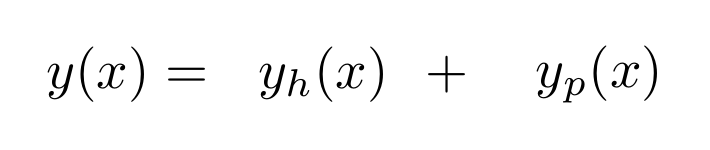
\begin{tikzpicture}
\node[scale=2] (a) at (0,0) {$y(x) = $};
\node[scale=2] (b) at (3,0) {$y_{h}(x) \:\:\: +$};
\node[scale=2] (c) at (6,0) {$y_{p}(x)$};
%\draw (2,0) -- (2,-1)[->,>=latex] -- (0,-1) ;
%\draw (3.5,0) -- (3.5,-1)[->,>=latex] -- (5,-1);
\end{tikzpicture}
\end{center}
\end{tcolorbox}

که 
$y_{h}(x)$
جواب عمومی بخش همگن و 
$y_{p}(x)$
جواب خصوصی بخش غیر همگن است

روش های مختلفی برای به دست آوردن جواب خصوصی بخش غیر همگن وجود دارد از جمله :
\begin{itemize}
	\item ضرایب نامعین
	\item  (operator) عملگر
	\item سری
\end{itemize}


\subsection{روش ضرایب نامعین}

از این روش فقط در مورد معادلات خطی با ضرایب ثابت می توان استفاده کرد ، قابل ذکر است r(x) باید تابعی باشد که در حالت های مختلف ذکر می شود .

در هر یک از حالات و یا ترکیبی از آنها $y_{p}$ به تناسب آن حالت به صورت یک تابع با ضرایب نامعین نوشته می شود .

پس از آن با قرار دادن
$y_{p}$
در معادله دیفرانسیل و هم ارز قرار دادن با سمت راست معادله ضرایب مجهول به دست می آید .



\subsubsection{حالت های مختلف r(x) که با روش ضرایب نامعین حل می شوند}


\subsubsection{r(x) به فرم یک چند جمله ای از درجه ی n باشد}


\begin{tcolorbox}
\begin{center}
\begin{tikzpicture}
\node[scale=2] (a) at (0,0) {$y_{p} = $};
\node[scale=2] (b) at (2.3,0) {$x^{m} \:\: \times$};
\node (c) at (7,0) {
(یک-چند-جمله-ای-کامل-از-درجه-ی-n)
};
%\draw (2,0) -- (2,-1)[->,>=latex] -- (0,-1) ;
%\draw (3.5,0) -- (3.5,-1)[->,>=latex] -- (5,-1);
\end{tikzpicture}
\end{center}
\end{tcolorbox}


m 
 تعداد ریشه های صفر معادله مشخصه می باشد


\subsubsection{مثال}

$$
y'' - 9y = 1
$$

به دست آوردن 
$y_{h}(x)$ :

\begin{align*}
&r^{2} - 9 = 0 \to r^{2} = 9 \to r = \pm 3 \\
&\to y_{h}(x) = c_{1}e^{3x} + c_{2}e^{-3x}
\end{align*}

به دست آوردن 
$y_{p}(x)$ :

\begin{align*}
&r(x) = 1 \to r(x) = 1 \times x^{0} \Rightarrow n = 0 \\
&\Rightarrow y_{p}(x) = x^{0} \times A \Rightarrow
\begin{cases}
y_{p}(x) = A \\
y'_{p} = 0 \\
y''_{p} = 0
\end{cases} \\
&\Rightarrow
y'' - 9y = 1 \to 0 - 9A = 1 \to A = - \frac{1}{9}
\end{align*}

جواب عمومی معادله ی دیفرانسیل مرتبه ی دوم خطی غیر همگن :

\begin{align*}
\Rightarrow y(x) = c_{1}e^{3x} + c_{2} e^{-3x} + - \frac{1}{9}
\end{align*}




\subsubsection{مثال}

$$
y'' - 4y = 2x^{2} - 3
$$

همانطور که میبینید r(x) چند جمله ای از درجه ی 2 می باشد .


به دست آوردن 
$y_{h}(x)$ :

\begin{align*}
&r^{2} - 4 = 0 \to r^{2} = 4 \to r = \pm 2 \\
&\Rightarrow y_{h}(x) = c_{1}e^{2x} + c_{2}e^{-2x}
\end{align*}

به دست آوردن 
$y_{p}(x)$ :

\begin{align*}
&y_{p}(x) = x^{0} \times ( Ax^{2} + Bx + C ) = ( Ax^{2} + Bx + C ) \\
&y'_{p}(x) = 2Ax + B \\
&y''_{p}(x) = 2A \\
\end{align*}


\begin{align*}
&y'' - 4y = 2x^{2} - 3 \\
&2A - 4 ( Ax^{2} + Bx + C ) = 2x^{2} - 3 \\
&2A - 4Ax^{2} - 4Bx - 4C = 2x^{2} - 3 \\
&-4Ax^{2} - 4Bx + 2A - 4C = 2x^{2} - 3 \\
&\Rightarrow 
\begin{cases}
-4A = 2 \Rightarrow A = - \frac{1}{2} \\
-4B = 0 \Rightarrow B = 0 \\
2A - 4C = -3 \Rightarrow -1 - 4C = -3 \Rightarrow -4C = -2 \Rightarrow C = \frac{1}{2}
\end{cases} \\
&\Rightarrow y_{p}(x) = -\frac{1}{2} x^{2} + \frac{1}{2}
\end{align*}

جواب عمومی :

$$
y(x) = c_{1}e^{2x} + c_{2}e^{-2x} - \frac{1}{2} x^{2} + \frac{1}{2}
$$



\subsubsection{مثال}

$$
y'' - y' = 2x
$$

چند جمله ای r(x) از درجه ی 1 می باشد .


به دست آوردن 
$y_{h}(x)$ :

\begin{align*}
y'' - y' = 0 \to r^{2} - r = 0 \to r( r - 1 ) = 0 \to 
\begin{cases}
r = 0 \\
r = 1 \\
\end{cases}
\end{align*}

\begin{align*}
\Rightarrow y_{h}(x) = c_{1}e^{0 \times x} + c_{2}e^{1 \times x} = c_{1} + c_{2}e^{x}
\end{align*}

به دست آوردن 
$y_{p}(x)$ :

\begin{align*}
&y_{p}(x) = x^{1} \times ( Ax + B ) = Ax^{2} + Bx \\
&y'_{p}(x) = 2Ax + B \\
&y''_{p}(x) = 2A \\
\end{align*}



\begin{align*}
&y'' - y' = 2x \to 2A - 2Ax - B = 2x \to -2Ax + 2A - B = 2x \\
&\Rightarrow \begin{cases}
-2A = 2 \to A = -1 \\
2A - B = 0 \to -2 - B = 0 \to B = -2
\end{cases}
\\
&\Rightarrow y_{p}(x) = -x^{2} - 2x
\end{align*}

جواب عمومی :

$$
\Rightarrow y(x) = c_{1} + c_{2}e^{x} - x^{2} - 2x
$$


\subsubsection{اگر 
r(x)
به صورت
$M(x)e^{tx}$
باشد }

 که در آن M(x) یک چند جمله ای از درجه ی n می باشد .

در این صورت جواب خصوصی پیشنهادی به صورت زیر می باشد .

\begin{tcolorbox}
\begin{center}
\begin{tikzpicture}
\node[scale=2] (a) at (0,0) {$y_{p} = $};
\node[scale=2] (b) at (2.3,0) {$x^{m} \: \times$};
\node[scale=2] (b) at (4.3,0) {$e^{tx} \: \times$};
\node (c) at (8.5,0) {
(یک-چند-جمله-ای-کامل-از-درجه-ی-n)
};
\end{tikzpicture}
\end{center}
\end{tcolorbox}


m تعداد t
در ریشه های معادله مشخصه می باشد .

\subsubsection{مثال}

$$
y'' - 5y' + 6y = 5e^{x}
$$

همانطور که میبینید ، داریم :

$$
5e^{1 \times x} \to t = 1
$$

به دست آوردن 
$y_{h}(x)$ :

\begin{align*}
&y'' - 5y' + 6y = 0 \to r^{2} - 5r + 6 = 0 \\
&\to \Delta = b^{2} - 4ac = (-5)^{2} - 4(6) = 25 - 24 = 1 \\
&r = \frac{ -b \pm \sqrt{\Delta} }{ 2a } = \frac{5 \pm 1}{2} = \begin{cases}
\frac{6}{2} = 3 \\
\frac{4}{2} = 2 \\
\end{cases}
\end{align*}

$$
\Rightarrow y_{h}(x) = c_{1}e^{3x} + c_{2}e^{2x}
$$


به دست آوردن 
$y_{p}(x)$ :

\begin{align*}
&y_{p} = x^{0} e^{x} ( A ) = A e^{x} \\
&y'_{p} = Ae^{x} \\
&y''_{p} = Ae^{x} 
\end{align*}

\begin{align*}
&y'' - 5y' + 6y = 5e^{x} \to Ae^{x} - 5Ae^{x} + 6Ae^{x} = 5e^{x} \\
\to \:\: &2Ae^{x} = 5e^{x} \\
\to \:\: &2A = 5 \to A = \frac{5}{2} \\
\end{align*}

جواب عمومی :

$$
y(x) = c_{1}e^{3x} + c_{2}e^{2x} + \frac{5}{2}e^{x}
$$


\subsubsection{مثال}


$$
y'' + 3y' + 2y = e^{-2x} 
$$

همانطور که میبینید ، داریم : 

$$
M(x) = 1 \quad t = -2
$$

به دست آوردن 
$y_{h}(x)$ :


\begin{align*}
&y'' + 3y' + 2y = 0 \to r^{2} + 3r + 2 = 0 \\
\to \:\: &\Delta = b^{2} - 4ac = 3^{2} - 4(2) = 9 - 8 = 1 \\
\to \:\: &r = \frac{ -b \pm \sqrt{\Delta} }{ 2a } = \frac{-3 \pm 1}{2} = \begin{cases}
- \frac{4}{2} = -2 \\
- \frac{2}{2} = -1 
\end{cases}
\end{align*}


به دست آوردن 
$y_{p}(x)$ :

\begin{align*}
y_{p}(x) &= x^{1} e^{-2x} ( A ) = Axe^{-2x} \\
y'_{p}(x) &= (Ae^{-2x} + -2e^{-2x} Ax) = Ae^{-2x} - 2Axe^{-2x} \\
y''_{p}(x) &= -2Ae^{-2x} - 2 ( Ae^{-2x} - 2 Axe^{-2x}) \\
& = -2Ae^{-2x} - 2 A e^{-2x} + 4Axe^{-2x} \\
& = -4A e^{-2x} + 4Axe^{-2x} 
\end{align*}


\begin{align*}
&y'' + 3y' + 2y = e^{-2x} \\
&\to -4Ae^{-2x} + 4Axe^{-2x} + 3 ( Ae^{-2x} - 2Axe^{-2x} ) + 2Axe^{-2x} = e^{-2x} \\
&\to -4Ae^{-2x} + 4Axe^{-2x} + 3Ae^{-2x} - 6Axe^{-2x} + 2Axe^{-2x} = e^{-2x} \\
&\to -Ae^{-2x} = e^{-2x} \to - A = 1 \to A = -1 \\
&\to y_{p}(x) = Axe^{-2x} \Rightarrow y_{p}(x) = -xe^{-2x}
\end{align*}

جواب عمومی معادله دیفرانسیل مرتبه ی دوم خطی غیر همگن :

$$
y(x) = c_{1}e^{-2x} + c_{2}e^{-x} - xe^{-2x}
$$

\chapter{تبدیل لاپلاس برای حل معادلات دیفرانسیل}

\section{تعریف تبدیل لاپلاس}

\begin{align*}
L \left[ f(t) \right] = F(s) = \int_{0}^{\infty}{e^{-st} \times f(t) dt}
\end{align*}

\begin{align*}
L \left[ f(t) \right] = F(s) 
\end{align*}

\begin{align*}
f(t) = L^{-1} \left[ F(s) \right]
\end{align*}



\subsubsection{مثال}

$$
f(t) = 1
$$

\begin{align*}
L [ 1 ] = F(s) &= \int_{0}^{\infty}{e^{-st} \times 1 \times dt} \\
&= \lim_{u \to \infty}{\int_{0}^{4}{e^{-st}dt}} \\
&= \lim_{u \to \infty}{ \left[ -\frac{1}{s} e^{-st} \right]_{0}^{u} } \\
&= \lim_{u \to \infty}{ \left[ - \frac{1}{s} e^{-su} - \left( - \frac{1}{s} e^{-s \times 0} \right) \right] } \\
&= \lim_{u \to \infty}{ \left[ - \frac{1}{s} e^{-su} + \frac{1}{s} \right] } \\
&= \frac{1}{s} 
\end{align*}


\subsubsection{نکته}

{
\LARGE
\begin{align*}
\lim_{x \to +\infty}{e^{x}} &= + \infty &\qquad \lim_{x \to +\infty}{e^{-x}} &= 0 
\end{align*}

\begin{align*}
\lim_{x \to -\infty}{e^{x}} &= 0 &\qquad \lim_{x \to -\infty}{e^{x}} &= + \infty 
\end{align*}
}



\subsubsection{مثال}

$$
f(t) = k
$$

\begin{align*}
L[k] = F(s) = \int_{0}^{+ \infty}{ e^{-st} \times k \times dt} = k \times \int_{0}^{+ \infty}{e^{-st} dt} = k \times \frac{1}{s} = \frac{k}{s}
\end{align*}

\begin{tcolorbox}
\begin{align*}
L[1] &= \frac{1}{s}   \\
L[k] &= \frac{k}{s} \\
L[ k \times f(t) ] &= k \times L[f(t)] \\
L[ f(t) + g(t) ] &= L[f(t)] + L[g(t)] \\
\end{align*}
\end{tcolorbox}



\subsubsection{مثال}

$$
f(t) = t
$$

\begin{align*}
L[t] = F(s) &= \int_{0}^{\infty}{e^{-st} . t dt} = \int_{0}^{\infty}{t e^{-st} dt} \\
&= \lim_{u \to \infty}{ \int_{0}^{u}{t e^{-st} dt} } \\
& f = t \qquad g' = e^{-st} \\
& f' = t \qquad g = - \frac{1}{s} e^{-st} \\
& \int{fg'} = fg - \int{f'g} \\
&= \lim_{u \to \infty}{ \left[ t \times - \frac{1}{s} e^{-st} \right]_{0}^{u} } - \int_{0}^{u}{- \frac{1}{s} e^{-st} dt } \\
& \lim_{u \to \infty}{ \left[ - \frac{t}{s} e^{-st} \right]_{0}^{u}  } + \frac{1}{s} \int_{0}^{u}{e^{-st}dt} \\
& \lim_{u \to \infty}{ - \frac{u}{s} e^{-st} - \left( - \frac{0}{s} \times e^{-s \times 0} \right) + \frac{1}{s} \times \left( - \frac{1}{s} e^{-st} \right)_{0}^{u} } \\
& \lim_{u \to \infty}{ \left[ - \frac{u}{s} e^{-st} + \frac{1}{s} \left( - \frac{1}{s} e^{-st} - \left( - \frac{1}{s} e^{-s \times 0} \right) \right) \right] } \\
&= \lim_{u \to \infty}{ \frac{1}{s} \times \frac{1}{s} } \\
& = \frac{1}{s^{2}}
\end{align*}


\begin{tcolorbox}
$$
L[t] = \frac{1}{s^{2}}
$$
\end{tcolorbox}



\subsubsection{مثال}


$$
f(t) = e^{at} \qquad t \geq 0
$$


\begin{align*}
L[e^{at}] = F(s) &= \int_{0}^{\infty}{e^{at} dt} = \int_{0}^{\infty}{e^{(a-s)t}dt} \\
&= \lim_{u \to \infty}{\int_{0}^{\infty}{e^{(a-s)t}dt}} \\
&= \lim_{u \to \infty}{\left[ \frac{1}{a-s} e^{(a-s)t} \right]_{0}^{u}}  \\
&= \lim_{u \to \infty}{\left[ \frac{1}{a-s} e^{(a-s)u} - \left( \frac{1}{a-s} e^{(a-s) \times 0} \right) \right]}
\end{align*}


$$
if \:\: s > 0 \to a < s \to a - s < 0 
$$

$$
\Rightarrow \frac{-1}{a-s} = \frac{1}{s-a} \:\: ; \:\: s > a
$$ 



\begin{tcolorbox}
$$
L \left[ e^{at} \right] = \frac{1}{s-a} \:\: ; \:\: s > 0
$$
\end{tcolorbox}



\subsubsection{مثال}

$$
f(t) = 8e^{2t} - e^{-t} + t 
$$

\begin{align*}
L[f(t)] &= L[8e^{2t} - e^{-t} + t] \\
&= L[8e^{2t}] - L[e^{-t}] + L[t] \\
&= 8 L[e^{2t}] - L[e^{-t}] + L[t] \\
&= 8 \times \frac{1}{s-2} - \frac{1}{s-(-1)} + \frac{1}{s^{2}} \\
&= \frac{8}{s-2} - \frac{1}{s+1} + \frac{1}{s^{2}}
\end{align*}




\subsubsection{مثال}

$$
f(t) = t^{a} \:\:\: ; \:\:\: a > -1
$$



\begin{tcolorbox}
$$
L[t^{a}] = \frac{a!}{s^{a+1}} \qquad \qquad L[t^{a}] = \frac{\Gamma{(a+1)}}{s^{a+1}}
$$
\end{tcolorbox}



\subsubsection{مثال}

$$
f(t) = \sin{at}
$$

\begin{tcolorbox}
$$
L[\sin{at}] = \frac{a}{s^{2} + a^{2}}
$$
\end{tcolorbox}

\subsubsection{مثال}

$$
f(t) = \cos{at}
$$

\begin{tcolorbox}
$$
L[\cos{at}] = \frac{s}{s^{2} + a^{2}}
$$
\end{tcolorbox}


\section{فرمولهای عکس لاپلاس}

\begin{latin}
\begin{center}
  \bgroup
  \def\arraystretch{3}%
  \begin{tabular}{ l | l  }
    $L^{-1}\left[ F(s) \right]$ & $F(s)$ \\
    \hline
    $L^{-1}\left[ \cfrac{1}{s} \right] = 1$ & $L[1] = \cfrac{1}{s}$ \\
    \hline
    $L^{-1}\left[ \cfrac{k}{s} \right] = k$ & $L[k] = \cfrac{k}{s}$ \\
    \hline
    $L^{-1}\left[ \cfrac{1}{s^{2}} \right] = t$ & $L[t] = \cfrac{1}{s^{2}}$ \\
    \hline
    $L^{-1}\left[ \cfrac{1}{s-a} \right] = e^{at}$ & $L[e^{at}] = \cfrac{1}{s-a} \:\: ; s > a$ \\
    \hline
    $L^{-1}\left[ \cfrac{a!}{s^{a+1}} \right] = t^{a}$ & $L[t^{a}] = \cfrac{a!}{s^{a+1}}$ \\
  \end{tabular}
  \egroup
\end{center}
\end{latin}







\section{عکس تبدیلات لاپلاس را محاسبه کنید}


\subsubsection{مثال}

$$
F(s) = \frac{1}{s^{2} + s - 2}
$$

\begin{align*}
&s^{2} + s - 2 = 0 \\
&\Delta = b^{2} - 4ac = 1^{2} - 4 ( -2 ) = 1 + 8 = 9 \\
&s = \frac{ -b \pm \sqrt{\Delta} }{2a} = \frac{-1 \pm 3}{2} = \begin{cases}
\frac{2}{2} = 1 \\
\frac{-4}{2} = -2 \\
\end{cases}
\end{align*}


\begin{align*}
\frac{1}{s^{2}+s-2} &= \frac{1}{(s-1)(s+2)} \\
&= \frac{A}{s-1} + \frac{B}{s+2} \\
&= \frac{As + 2A + Bs - B}{(s-1)(s+2)} \\
&= \frac{(A+B)s + 2A - B}{(s-1)(s+2)}
\end{align*}

\begin{align*}
\begin{cases}
A + B = 0 \to A = - B \\
2A - B = 1 \to -2B - B = 1 \to -3B = 1 \to B = - \frac{1}{3} \to A = \frac{1}{3}
\end{cases}
\end{align*}

\begin{align*}
F(s) &= \frac{\frac{1}{3}}{s - 1} + \frac{- \frac{1}{3}}{s+2} \\
L^{-1}\left[ F(s) \right] &= L^{-1}\left[ \frac{\frac{1}{3}}{s - 1} \right] + L^{-1}\left[ \frac{- \frac{1}{3}}{s+2} \right] \\
&= \frac{1}{3} L^{-1}\left[ \frac{1}{s-1} \right] + (- \frac{1}{3} ) L^{-1}\left[ \frac{1}{s+2} \right] \\
&= \frac{1}{3} e^{t} - \frac{1}{3} e^{-2t} 
\end{align*}


\subsubsection{کاربرد تبدیل لاپلاس}

بعد از معرفی تبدیل لاپلاس و عکس تبدیل لاپلاس برای حل معادلات دیفرانسیل از آنها استفاده می کنیم .

\begin{enumerate}
	\item تبدیل لاپلاس مشتق
	\item تبدیل لاپلاس انتگرال
	\item مشتق تبدیل لاپلاس
	\item انتگرال تبدیل لاپلاس
\end{enumerate}

از 4 حالت فوق ، فعلاً به شماره ی 1 می پردازیم .


\section{تبدیل لاپلاس مشتق}

\subsection{حالت اول}
اگر تبدیل لاپلاس مشتق مرتبه ی اول را حساب کنیم ، به فرم زیر تعیین می شود .

\begin{tcolorbox}
$$
L \left[ f'(t) \right] = s L\left[ f(t) \right] - f(0)
$$
\end{tcolorbox}


\subsubsection{
به کمک تبدیل لاپلاس جواب مسئله با شرط اولیه ی زیر را تعیین کنید
}

$$
y' + 2y = 4t \:\: ;  \:\: y(0) = 5
$$


\begin{align*}
L \left[ y' + 2y \right] &= L \left[ 4t \right] \\
L \left[ y' \right] + 2 L \left[ y \right] &= 4 L \left[ t \right] \\
\end{align*}

\begin{tcolorbox}
$$
L[y'] = sL[y] - y(0)
$$
\end{tcolorbox}

\begin{align*}
sL[y] - y(0) + 2L[y] &= 4L[t] \\
(s+2) L [y] - 5 &= 4 \times \frac{1}{s^{2}} \quad ; L[y] = Y(s) \\
(s+2) Y(s) &= \frac{4}{s^{2}} + 5 \\
Y(s) &= \frac{4}{s^{2}(s+2)} + \frac{5}{s+2}
\end{align*}


\begin{tcolorbox}
$$
L[y(t)] = Y(s) \qquad L^{-1}[Y(s)] = y(t)
$$
\end{tcolorbox}


\begin{align*}
\frac{4}{s^{2}(s+2)} &= \frac{A}{s} + \frac{B}{s^{2}} + \frac{C}{s+2} \\
&= \frac{As + B}{s^{2}} + \frac{C}{s+2} \\
&= \frac{(As+B)(s+2) + Cs^{2}}{s^{2}(s+2)} \\
&= \frac{As^{2} + 2As + Bs + 2B + Cs^{2}}{s^{2}(s+2)} \\
&= \frac{(A+C)s^{2} + (2A+B)s + 2B}{s^{2}(s+2)}
\end{align*}


\begin{align*}
2B &= 4 \to B = 2 \\
2A + 2 &= 0 \to A = -1 \\
A + C &= 0 \to C = 1 \\
\end{align*}

$$
\to \frac{4}{s^{2}(s+2)} = \frac{-1}{s} + \frac{2}{s^{2}} + \frac{1}{s+2}
$$



\begin{align*}
L^{-1}[Y(s)] &= L^{-1}\left[ \frac{4}{s^{2}(s+2)} \right] + L^{-1}\left[ \frac{5}{s+2} \right] \\
&= L^{-1}\left[ \frac{-1}{s} + \frac{2}{s^{2}} + \frac{1}{s+2} \right] + 5 \times L^{-1}\left[ \frac{1}{s+2} \right] \\
&= -1 + 2t + e^{-2t} + 5 \times e^{-2t} 
\end{align*}



\subsubsection{مثال}

$$
y' - y = \sin{t} - \cos{t} + e^{t} \:\:\: ; \:\:\: y(0) = -2
$$



\begin{align*}
L[y' - y] &= L[\sin{t} - \cos{t} + e^{t}] \\
L[y'] - L[y] &= L[\sin{t}] - L[\cos{t}] + L[e^{t}] \\
\end{align*}


\begin{tcolorbox}
$$
L[y'] = sL[y] - y(0)
$$
\end{tcolorbox}


\begin{align*}
sL[y] - y(0) - L[y] &= L[\sin{t}] - L[\cos{t}] + L[e^{t}] \\
(s-1) L [y] + 2 &= \frac{a}{s^{2} + a^{2}} - \frac{s}{s^{2} + a^{2}} + \frac{1}{s-1} \\
(s-1) L [y] &= \frac{a}{s^{2} + a^{2}} + - \frac{s}{s^{2} + a^{2}} + \frac{1}{s-1} - 2 \\
L [y] &= \frac{a}{(s^{2} + a^{2})(s-1)} - \frac{s}{(s^{2} + a^{2})(s-1)} + \frac{1}{(s-1)^{2}} - \frac{2}{s-2} \\
\end{align*}

\begin{tcolorbox}
$$
\sin{t} \Rightarrow a = 1 \qquad \qquad \cos{t} \Rightarrow a = 1
$$
\end{tcolorbox}


\begin{align*}
L[y] &= \frac{1}{(s-1)(s^{2}+1)} - \frac{s}{(s-1)(s^{2}+1)} + \frac{1}{(s-1)^{2}} - \frac{2}{s-1}
\end{align*}

\begin{tcolorbox}
$$
L[te^{t}] = \frac{1}{(s-1)^{2}}
$$
\end{tcolorbox}


\begin{align*}
Y(s) = \frac{1}{(s-1)(s^{2}+1)} - \frac{s}{(s-1)(s^{2}+1)} + \frac{1}{(s-1)^{2}} - \frac{2}{s-1}
\end{align*}


\begin{align*}
\frac{1}{(s-1)(s^{2}+1)} &= \frac{A}{s-1} + \frac{Bs + C}{s^{2} + 1} \\
&= \frac{A(s^{2}+1) + (Bs + C)(s-1)}{(s-1)(s^{2}+1)} \\
&= \frac{As^{2} + A + Bs^{2} - Bs + Cs - C}{(s-1)(s^{2}+1)} \\
&= \frac{(A+B)s^{2} + (C-B)s + A - C}{(s-1)(s^{2}+1)}
\end{align*}


\begin{align*}
&A - C = 1 \to A = C + 1 \to - B = B + 1 \to 2B = -1 \to B = \frac{-1}{2} \\
&C - B = 0 \to C = B \to C = \frac{-1}{2} \\ 
&A + B = 0 \to A = -B \to A = \frac{1}{2} 
\end{align*}

\begin{align*}
\Rightarrow \frac{1}{(s-1)(s^{2}+1)} = \frac{\frac{1}{2}}{s-1} + \frac{\frac{-1}{2} s - \frac{1}{2}}{s^{2} + 1}
\end{align*}



\begin{align*}
\frac{s}{(s-1)(s^{2}+1)}  &= \frac{A}{s-1} + \frac{Bs + C}{s^{2} + 1} \\
&= \frac{(A+B)s^{2} + (C-B)s + A - C}{(s-1)(s^{2}+1)}
\end{align*}


\begin{align*}
&A - C = 0 \to A = C \to C = \frac{1}{2} \\
&A + B = 0 \to A = - B \\
&C - B = 1 \to C = B + 1 \to A = B + 1 \\
&\to -B = B + 1 \to -2 B = 1 \to B = \frac{-1}{2} \\
&\to A = \frac{1}{2}
\end{align*}



\begin{align*}
\frac{s}{(s-1)(s^{2}+1)}  = \frac{\frac{1}{2}}{s-1} + \frac{\frac{-1}{2} s + \frac{1}{2}}{s^{2} + 1}
\end{align*}

\begin{align*}
L^{-1}[Y(s)] &= L^{-1}\left[ \frac{1}{(s-1)(s^{2}+1)} \right] - L^{-1}\left[ \frac{s}{(s-1)(s^{2}+1)} \right] + L^{-1}\left[ \frac{1}{(s-1)^{2}} \right] - L^{-1}\left[ \frac{2}{s-1} \right] \\
&= L^{-1}\left[ \frac{\frac{1}{2}}{s-1} + \frac{\frac{-1}{2} s - \frac{1}{2}}{s^{2} + 1}  \right] - L^{-1}\left[ \frac{\frac{1}{2}}{s-1} + \frac{\frac{-1}{2} s + \frac{1}{2}}{s^{2} + 1} \right] + L^{-1}\left[ \frac{1}{(s-1)^{2}} \right] - L^{-1}\left[ \frac{2}{s-1} \right] \\
&= - L^{-1}\left[ \frac{1}{s^{2}+1} \right] + L^{-1}\left[ \frac{1}{(s-1)^{2}} \right] - L^{-1}\left[ \frac{2}{s-1} \right] \\
&= - \sin{t} + te^{t} - 2e^{t}
\end{align*}











\end{document}